\chapter{The evolutionary origins of phenotypic plasticity}
\label{chapter:evolutionary-origins-of-plasticity}



\def \lineageVisualizationURL{https://lalejini.com/evo-origins-of-phenotypic-plasticity-web/}

% Thoughts:
% - It really shows that this chapter is my first publication. A little clunky overall.
% - I definitely did *not* yet know how to manage experiment code, data, and analyses well. Was *way* more challenging than it needed to be to regenerate figures.

\noindent
Authors: Alexander Lalejini and Charles Ofria \\
This chapter is adapted from ~\citep{lalejini_evolutionary_2016}, which underwent peer review and appeared in the proceedings of the 2016 Artificial Life Conference. 

\section{Introduction}
\label{chapter:origins-of-plasticity:sec:introduction}

% What is phenotypic plasticity and why is it important?
Phenotypic plasticity is the capacity for a genotype to express different phenotypes in response to different environmental conditions \citep{ghalambor_behavior_2010} and is ubiquitous throughout nature. 
Phenotypic plasticity is central to many complex traits and developmental patterns found in nature and often serves as a key strategy employed by organisms to respond to spatially and temporally variable environments \citep{bradshaw_evolutionary_1965,murren_constraints_2015}.
For example, \textit{Daphnia pulex} use plasticity to differentially invest in morphological defenses during development, depending on the presence of predators in their local environment \citep{black_demographic_1990}. 
Genetically homogeneous cells in a developing multicellular organism leverage their capacity for phenotypic plasticity to coordinate their expression patterns through environmental signals \citep{schlichting_origins_2003}.
Thus, understanding the evolution of plasticity is an important step toward a deeper understanding of biological complexity. 

Phenotypic plasticity also has practical applications in the field of evolutionary computation where evolution by natural selection is harnessed to solve challenging computational and engineering problems. 
In many realistic problem domains, conditions are noisy or cyclically change. 
Plasticity enables solutions to dynamically respond to changing problem conditions and be robust to noise. 
Both the biological and evolutionary computation domains motivate the following questions: 
(1) Under what conditions does phenotypic plasticity evolve? 
And (2), what are the evolutionary stepping stones for phenotypic plasticity? 

% What are the conditions for phenotypic plasticity?
Ghalambor \textit{et al.} identify four conditions that are necessary for phenotypic plasticity to evolve: 
(1) populations are exposed to temporally or spatially varying environments, 
(2) the environments are differentiable by reliable signals, 
(3) different environments favor different phenotypes, and 
(4) no single phenotype can exhibit high fitness across all environments \citep{ghalambor_behavior_2010}. 
Theoretical and empirical findings support that phenotypic plasticity can evolve under these conditions in both natural and artificial systems \citep{clune_investigating_2007,goldsby_evolution_2010,goldsby_evolutionary_2014,hallsson_selection_2012,nolfi_phenotypic_1994}.

% Process by which phenotypic plasticity evolves, motivate digital evolution
In addition to exploring the conditions that facilitate the evolutionary origin of phenotypic plasticity, it is also important to explore the step-by-step process out which plasticity actually evolves. 
What are the reoccurring themes as evolution progresses toward more plastic strategies?
Are there genotypic or phenotypic patterns present in lineages leading to phenotypically plastic organisms? 
These types of questions are especially difficult to address in laboratory systems due to the slow pace of natural evolution, imperfections in lineage tracking, and the difficulty of acquiring high-resolution data on genotypes and phenotypes. 
As such, artificial life systems are the most effective way to observe and analyze the process by which phenotypic plasticity evolves.

% What did we do? 
Here, we use the Avida Digital Evolution Platform \citep{ofria_avida:_2009} to explore the process by which phenotypic plasticity evolves in a fluctuating environment. 
First, we investigate how environmental factors impact the evolution of phenotypic plasticity.
Specifically, we evaluate how mutation rate and environment fluctuation rate affect the evolution of adaptive plasticity.
Next, we identify the evolutionary stepping stones in the evolution of adaptive phenotypic plasticity: do digital organisms evolve to express traits unconditionally before evolving to conditionally express them as a function of their environment, and do sub-optimal forms of plasticity evolve before more optimal forms of plasticity? 
We empirically test whether such intermediate evolutionary stepping stones are important to the evolution of adaptive plasticity. 
Finally, we examine alternative evolutionary strategies to phenotypic plasticity in fluctuating environments and see evidence for bet-hedging strategies that use mutationally induced phenotype switching as a substitute for sensory-dependent plasticity.   
\section{Methods}
\label{chapter:origins-of-plasticity:sec:methods}

\subsection{The Avida Digital Evolution Platform}
\label{chapter:origins-of-plasticity:sec:methods:avida}

The Avida software platform provides a computational instance of evolution and enables researchers to experimentally test hypotheses about evolution that would otherwise be difficult or impossible to test in natural systems \citep{ofria_avida:_2009}. 
Avida has a robust genetic encoding: all possible genetic sequences are well-defined in any context \citep{ofria_avida:_2009}. 
Avida has also been shown to be capable of evolving to use a wide range of capabilities \citep{bryson_understanding_2013}, making it an ideal choice for studying phenotypic plasticity. 
Here, we provide a brief overview of Avida as it is relevant to this work. 
For a more detailed description of the Avida software platform, see \citep{ofria_avida:_2009}.

\subsubsection{Digital Organisms}
\label{chapter:origins-of-plasticity:sec:methods:avida:organisms}

% Overview of Avida
Populations in Avida are made up of self-replicating computer programs (digital organisms) that compete for space in a finite, toroidal grid. 
Each of these digital organisms is defined by a sequence of instructions (\textit{i.e.}, its genotype), virtual hardware to execute the instructions, and a position on the grid. 
The instruction set of Avida is Turing-Complete and enables organisms to perform basic computations, control their own execution flow, and replicate. 
An organism's virtual hardware (Figure \ref{chapter:origins-of-plasticity:fig:avida-virtual-cpu}) includes components such as a central processing unit (CPU), registers used for computation, input and output buffers, and memory stacks. 
Organisms replicate asexually by copying themselves line-by-line and dividing; however, an organism's copy instruction is imperfect, which can result in mutated offspring.


\begin{figure*}[!t]
  \centering
  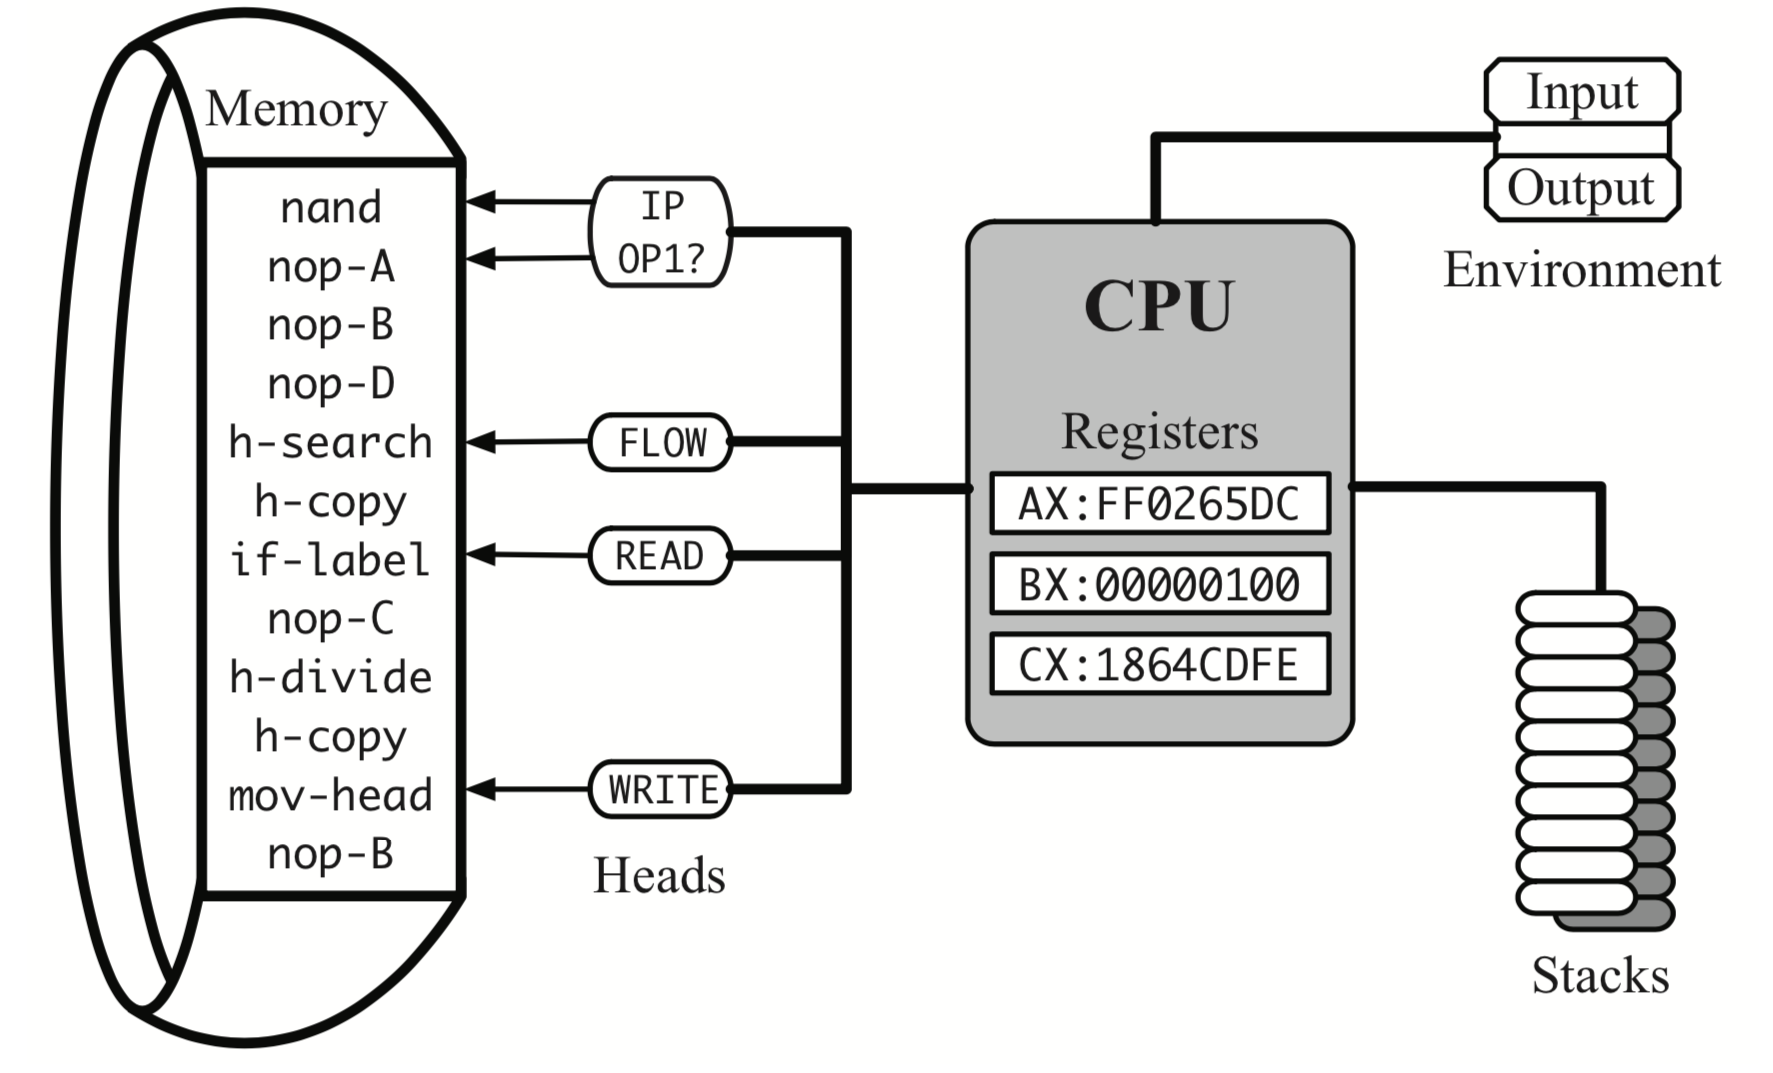
\includegraphics[width=\textwidth]{chapters/02-evolutionary-origins-of-plasticity/media/avida-virtual-cpu.png}
  \caption{\small 
    \textbf{A visual representation of the default virtual hardware used by organisms in Avida. }
    Original figure from \citep{ofria_avida:_2009}.
  }
  \label{chapter:origins-of-plasticity:fig:avida-virtual-cpu}
\end{figure*}

% Metabolism, competition
Organisms can gain additional CPU cycles by performing tasks---such as mathematical computations---to improve their metabolic rate. 
An organism's metabolic rate determines how rapidly it can execute its genome; a higher metabolic rate allows an organism to replicate faster. 
Initially, an organism's metabolic rate is roughly proportional to its genome length; however, the organism's metabolic rate can be adjusted when the organism completes a task. 
In this way, we can differentially reward or punish the performance of different tasks.

When an organism successfully replicates, its offspring is placed in a random location in the world, replacing the organism formerly occupying that location. 
In this way, becoming a more efficient replicator in Avida is advantageous in the competition for space. 
The combination of competition for replication efficiency and heritable variation due to imperfect copying during the replication process results in evolution by natural selection. 

\subsubsection{Sensing in Avida}
\label{chapter:origins-of-plasticity:sec:methods:avida:sensing}

% Sensing in Avida
In a typical Avida run, organisms must execute an instruction called \code{IO} to output the result of a computation. 
That output is analyzed to determine if any tasks have been performed, and if so, the organism is appropriately rewarded or punished. 
However, in this default scenario, organisms cannot sense the result, even after the task has been performed. 
To provide organisms with a mechanism to sense their environment, we added an \code{IO-Sense} instruction to the set of available instructions\footnote{
\code{IO-Sense} is based on the \code{IO-Feedback} instruction implemented in \citep{clune_investigating_2007}, which worked exactly as the default \code{IO} instruction, but provided the organism with feedback on the result.
As such, an organism must first do a particular task once---and potentially get punished---to sense whether or not the task is beneficial with the \code{IO-Feedback} instruction.
}.

The \code{IO-Sense} instruction simulates \code{IO} and provides the organism with feedback on what would have happened if the organism had executed an \code{IO} instruction instead. 
This separation of \code{IO} performance and sensing allows organisms to determine whether or not a particular task is being punished without the risk of punishment, lowering the potential cost of sensing. 
If an \code{IO} operation would have resulted in a punishment, a -1 is added to the top of the organism's stack memory; if it would have resulted in a reward, a 1 is placed there. 
If an \code{IO} operation would have resulted in neither a reward nor a punishment, a 0 is placed on the organism's stack memory. 
In this way, organisms can sense whether or not a particular task is being rewarded or punished in their current environment and then react accordingly.  

\subsubsection{Identifying Phenotypic Plasticity in Avida}
\label{chapter:origins-of-plasticity:sec:methods:avida:identifying-plasticity}

% identifying phenotypic plasticity in avida 
We define a phenotypically plastic organism in Avida as an organism that leverages sensory information to alter their phenotype based on the environment.
We restrict the definition of an organism's phenotype to the set of unique tasks it performs in the given environment. 
We do not consider how many times an organism performs a particular task in a given environment, but only whether the organism does the task at all. 
Thus, to be phenotypically plastic, an organism must express a different task profile (\textit{i.e.}, perform different tasks) in different environments. 

\subsection{Experimental Design}
\label{chapter:origins-of-plasticity:sec:methods:experimental-design}

% Lead-in
To explore the evolutionary history of phenotypically plastic organisms, we used an experimental design based on \citep{clune_investigating_2007}. 

% Environment
\subsubsection{Environments}
\label{chapter:origins-of-plasticity:sec:methods:experimental-design:environments}

We constructed two experimental environments named ENV-NAND and ENV-NOT.
In ENV-NAND, organisms were rewarded for performing the NAND logical task but were punished for performing the NOT logical task. 
Conversely, in ENV-NOT, organisms were rewarded for performing the NOT logical task but were punished for performing the NAND logical task. 
In each of our experimental treatments, we cycled between these two environmental conditions. 
In this way, genotypes with the capacity to sense the current environment and express the appropriate task had a competitive advantage over non-plastic organisms. 

\subsubsection{Phenotypes}
\label{chapter:origins-of-plasticity:sec:methods:experimental-design:phenotypes}

% Possible phenotypes
Given our simple definition of a phenotype, there are only four possible phenotypes in each of the two previously described environments: 
(1) perform only NAND, 
(2) perform only NOT, 
(3) perform both NAND and NOT, 
and (4) perform neither NAND nor NOT. 
When considering an organism's phenotype across both ENV-NAND and ENV-NOT, there are sixteen possible combinations. 
We enumerate these phenotypes in Figure \ref{chapter:origins-of-plasticity:fig:task-profiles}. 
Of these sixteen possible phenotypes, only four express the identical task profile in both environments; the other twelve profiles all exhibit some form of plasticity. 
The optimal form of plasticity is to perform only the NAND task in ENV-NAND and to perform only the NOT task in ENV-NOT; any other form of plasticity is sub-optimal. 
There are five possible phenotypes that leverage plasticity to perform punished tasks instead of rewarded tasks in a given environment; we did not expect these forms of phenotypic plasticity to be successful. 


% Table that enumerates possible phenotypic states
\begin{figure*}[!ht]
  \centering 
  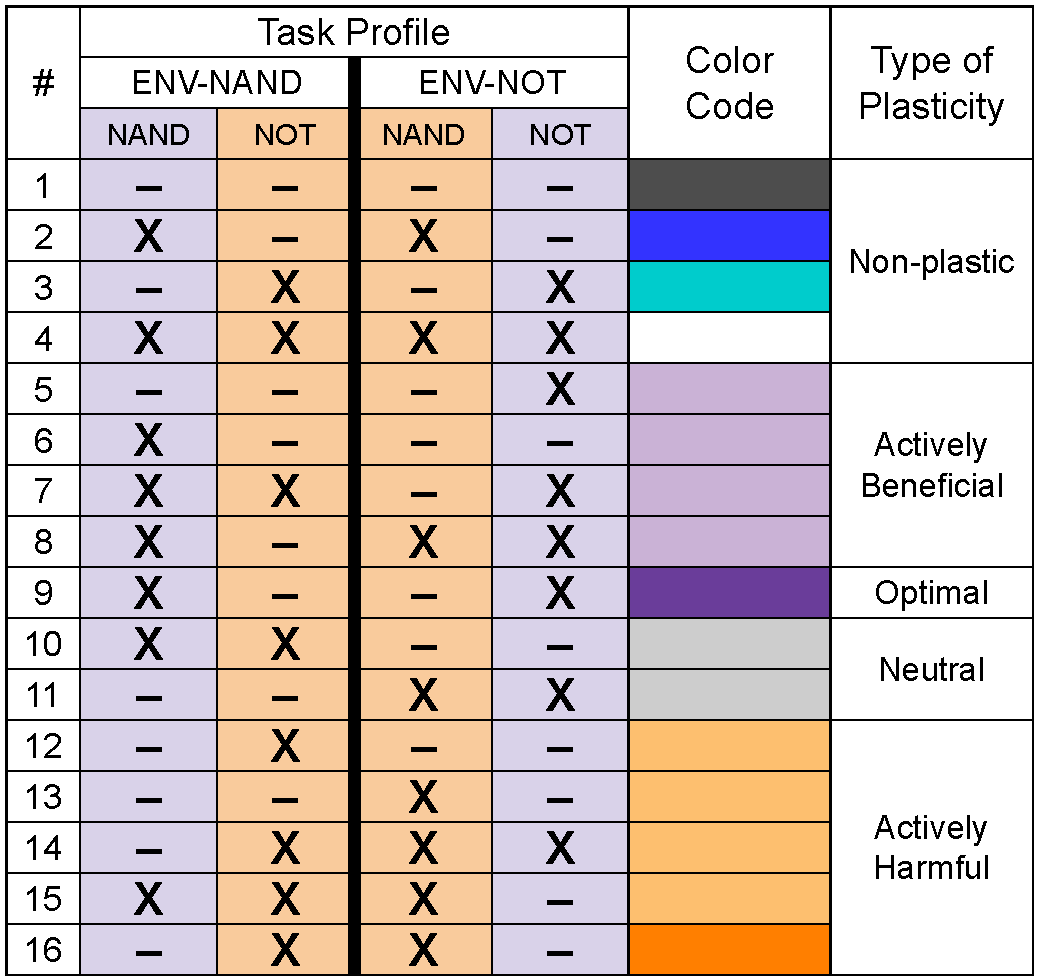
\includegraphics[width=0.75\columnwidth]{chapters/02-evolutionary-origins-of-plasticity/media/task-profiles.pdf}
  \caption{\small 
  \textbf{Enumeration of all possible complete phenotypes.}
  Each row represents a distinct phenotype. 
  An `X' indicates that the associated task is performed in the specified environment, while a `--' indicates that the task is not performed. 
  For each environment, the column of the rewarded task is highlighted in light purple, and the column of the punished task is highlighted in light orange. 
  An `X' in a reward column or a `--' in the punished column is optimal. 
  Each phenotype has a color code, which is used in our lineage visualization visualizations.  
  Note that the first four rows are non-plastic phenotypes, rows 5--8 exhibit partially beneficial plasticity, and row 9 is optimally beneficial.  
  Rows 10--11 are neutral non-adaptive plasticity, while rows 12--16 are detrimental forms of plasticity.}
  \label{chapter:origins-of-plasticity:fig:task-profiles}
\end{figure*}

\subsubsection{Treatments}
\label{chapter:origins-of-plasticity:sec:methods:experimental-design:treatments}

% Experimental treatments
Our experimental design consisted of five treatments and a control: 
(1) a baseline treatment with a moderate point-mutation rate and environmental-cycle length, 
(2) a low-mutation-rate treatment, 
(3) a high-mutation-rate treatment, 
(4) a short-environment-cycle-length treatment, 
(5) a long-environment-cycle-length treatment, 
and (6) a control where both NAND and NOT were rewarded and the environment did not fluctuate. 
See Table \ref{chapter:origins-of-plasticity:table:treatments} for treatment details.

We created the baseline treatment to produce phenotypically plastic organisms for lineage analysis. 
We limited the population size to 3600 organisms and seeded the world with an ancestral genotype capable only of self-replication.
We then evolved populations for 100,000 updates\footnote{
An update in Avida is an experimental length of time. One update is defined as the amount of time it takes for the average organism to execute 30 instructions (see \citep{ofria_avida:_2009} for more details).
} in Avida. 
We imposed a 0.0075 probability of point-mutation per instruction copied, as well as a 0.05 probability for each of single-instruction insertion and deletion per genome copied. 
We fluctuated the current environment between ENV-NAND and ENV-NOT every 100 updates in the baseline treatment. 
We ran 50 replicates of each treatment, including the control. 

% Table 'bout treatments
\begin{table}
\renewcommand{\arraystretch}{1.5}
  \centering
  \small
  \begin{tabular}{| >{\raggedright} p{0.3\columnwidth} |r | r| }
    \hline
    \centering \textbf{Treatment} & \multicolumn{1}{>{\raggedright\arraybackslash}p{0.25\columnwidth}|}{\centering \textbf{Point-mutation Rate}} & \multicolumn{1}{>{\raggedright\arraybackslash}p{0.30\columnwidth}|}{\centering \textbf{Environment Cycle Length }}
    \\ \hline 
    Baseline &  0.0075 &  100 updates  
    \\ \hline 
    Low Mutation Rate &  0.0025 & 100 updates 
    \\ \hline 
    High Mutation Rate &  0.0125 &  100 updates 
    \\ \hline
    Short Environment Cycle Length & 0.0075 &  50 updates 
    \\ \hline 
    Long Environment Cycle Length & 0.0075 &  200 updates 
    \\ \hline 
  \end{tabular}
  \caption{\small 
  \textbf{Differences among the five experimental treatments. }
  Point-mutation rate is given as mutations per instruction copied.
  Environment cycle length describes the length of time (in updates) an environment is active before toggling to the alternative environment.
  }
  \label{chapter:origins-of-plasticity:table:treatments}
\end{table}

\subsubsection{Lineage Visualization}
\label{chapter:origins-of-plasticity:sec:methods:experimental-design:lineage-visualization}

To explore evolutionary strategies evolved in fluctuating environments, we visualized the lineages of evolved genotypes as vertical bars where time (in updates) proceeds from top to bottom beginning with the lineage's original ancestor genotype.
Any given genotype on the lineage must express one of the sixteen possible phenotypes enumerated in Figure \ref{chapter:origins-of-plasticity:fig:task-profiles}.
At each point in time, the color of the visualized lineage corresponds to the color representing the phenotype expressed by the lineage at that point in time. 
For example, because the ancestral organism is capable only of self-replication, all visualized lineages should show that the original ancestor's phenotype performed neither the NAND task nor the NOT task. 
In addition to the visualized lineages, we indicate the actual environmental conditions experienced by the evolving populations at each point in time by the color of the vertical axis. 
This type of visualization allows us to display the phenotypic states traversed by any given lineage, allowing us to explore evolutionary strategies leveraged by all evolved lineages.

\section{Results and Discussion}

\subsection{What conditions promote the evolution of phenotypic plasticity?}

Ghalambor \textit{et al.} identified four environmentally-dependent requirements for the evolution of phenotypic plasticity
\citep{ghalambor_behavior_2010}. 
Our experimental design conforms to these conditions, enabling us to test their validity and relative importance. 
The oscillation between ENV-NAND and ENV-NOT provides temporal variation. 
The IO-Sense instruction reliably indicates the current environment. 
The two environments favor opposing phenotypic traits, and the only way for an individual organism to achieve a high fitness in both environments is to alter its phenotypic expression. 
Given the existing theoretical and empirical support for these conditions, we expected to see the evolution of phenotypic plasticity in each of our experimental treatments. 
However, we were unsure of the impact of altering environmental factors such as mutation rate and environment fluctuation rate. 

% Report plasticity results. 
At the end of the experiment, we extracted the dominant (most abundant) genotype from the population of each replicate.
We tested these genotypes in both ENV-NAND and ENV-NOT and recorded each genotype's expressed phenotype across both environments. 
In Table \ref{chapter:origins-of-plasticity:table:evolutionary-outcomes}, we report the number of replicates in which the dominant genotype at the end of the experiment was plastic and the number of replicates in which the dominant genotype was optimally plastic. 
Note that for these results we only evaluated the most abundant genotype at the end of the experiment. 
An ancestor of the evaluated genotype may have been plastic, but if that plasticity was not maintained in the lineage, we did not count it in Table \ref{chapter:origins-of-plasticity:table:evolutionary-outcomes}. 

% More specifically report results
As expected, the capacity for phenotypic plasticity evolved in each experimental treatment; in 31 of the 50 baseline treatment replicates, phenotypic plasticity was present in the final dominant organism. 
None of the final dominant genotypes from the control replicates were phenotypically plastic. 
In all control replicates, the dominant genotype performed both the NAND and NOT tasks unconditionally. 
Our results are consistent with existing theoretical and empirical work, supporting the validity of the conditions likely to facilitate the evolution of phenotypic plasticity \citep{clune_investigating_2007,ghalambor_behavior_2010,hallsson_selection_2012,nolfi_phenotypic_1994}. 

\begin{table*}[t]
\renewcommand{\arraystretch}{1.5}
	\centering
    \small
    \begin{tabulary}{\textwidth}{| l | r | r | r | r | r |}
      \hline 
      \multicolumn{1}{| c |}{\centering \textbf{Treatment}} &
      \multicolumn{2}{ c |}{\centering \textbf{Plastic Replicates}} &
      \multicolumn{2}{ p{0.25\textwidth}|}{\centering \textbf{Unconditional Precedes Conditional}} & \multicolumn{1}{p{0.20\textwidth}|}{\centering \textbf{Sub-optimal Precedes Optimal}} \\
      \cline{2-5}
      & \multicolumn{1}{p{0.1\textwidth} |}{\centering Total} & \multicolumn{1}{p{0.1\textwidth} |}{\centering Optimal$^{*}$} & \multicolumn{1}{p{0.1\textwidth} |}{\centering NAND Task} & \multicolumn{1}{p{0.1\textwidth} |}{\centering NOT Task} & \\
      \hline 
      Baseline 						 & 31 (62\%) & 17 (34\%) & 31 (100\%)   & 28 (90.3\%) & 16 (94.1\%) \\
      \hline 
      Low Mutation Rate 			 & 38 (76\%) & 30  (60\%) & 34 (89.5\%) & 35 (92.1\%) & 30 (100\%) \\
      \hline 
      High Mutation Rate  			 & 25 (50\%) & 11  (22\%) & 25 (100\%)  & 24 (96\%)  & 10 (90.9\%) \\
      \hline 
      \parbox[t]{0.2\textwidth}{Short Environment Cycle Length} & 36 (72\%) & 18  (36\%) & 33 (91.7\%) & 28 (77.8\%) & 18 (100\%) \\
      \hline 
      \parbox[t]{0.2\textwidth}{Long Environment Cycle Length}  & 16 (32\%) & 10  (20\%) & 14 (87.5\%) & 16 (100\%)  & 9 (90\%) \\
      \hline 
      Control						 & 0 (0\%) & 0 (0\%) & \multicolumn{1}{c|}{--} & \multicolumn{1}{c|}{--} & \multicolumn{1}{c|}{--} \\
      \hline 
    \end{tabulary}
    \begin{tablenotes}
          \item[*] $^{*}$\small{Optimal is defined as the complete phenotype that only performs the rewarded task in each environment.}
    \end{tablenotes}
    \caption{\small 
    \textbf{A summary of evolutionary outcomes across all five experimental treatments and control.}
    Plastic Replicates indicates the number of replicates (out of 50 per treatments) in which the final dominant genotype was plastic at all (Total) and perfectly plastic (Optimal).  
    Unconditional Precedes Conditional indicates the number of times the NAND task and NOT task were expressed unconditionally before eventually evolving to be express conditionally (out of total plastic).  
    Finally, Sub-optimal Precedes Optimal indicates how many runs had an imperfect form of plasticity before eventually evolving to be optimally plastic (out of total optimally plastic).
    }
    \label{chapter:origins-of-plasticity:table:evolutionary-outcomes}
\end{table*}

\subsection{How do environmental factors impact the evolution of phenotypic plasticity?}

While our results show phenotypic plasticity can evolve under the conditions identified in \citep{ghalambor_behavior_2010}, how do mutation rate and fluctuation rate affect the evolution of phenotypic plasticity under these conditions? 
We found compelling results for both mutation rate and environmental cycle length. 

\subsubsection{Mutation Rate}

While only of borderline statistical significance ($p = 0.058$ using Fisher's Exact Test with Bonferroni corrections for multiple comparisons; all statistics were done in R version 3.2.2 \citep{r_core_team_2016}), our results trend such that populations at lower mutation rates appear more likely to evolve phenotypic plasticity than do populations at higher mutation rates. 
The most abundant genotypes exhibited some plasticity in 38/50 runs at a low mutation rate, 31/50 at the baseline mutation rate, and 25/50 and the high mutation rate.  
While higher mutation rates increase genetic variation from one generation to the next, most mutations that have phenotypic effects are deleterious \citep{sniegowski_evolution_2000}. 
Thus, at higher mutation rates, the elevated influx of deleterious mutations could increase the difficulty of maintaining the necessary genetic machinery for phenotypic plasticity.
Qualitative evidence for this effect can be seen in the time-sliced visualized lineages of final dominant, non-plastic genotypes from the high-mutation-rate treatment (Figure \ref{chapter:origins-of-plasticity:fig:high-mut-lineages}) where lineages traverse states of plasticity for some time before reverting back to states of non-plasticity\footnote{
For fully interactive visualizations of evolved lineages from all treatments, see \url{https://lalejini.com/evo-origins-of-phenotypic-plasticity-web/}
}.
Furthermore, more phenotypic shifts in general increase the probability of quickly finding an appropriate non-plastic phenotype after each environmental change.

\begin{figure*}[ht]
  \centering
  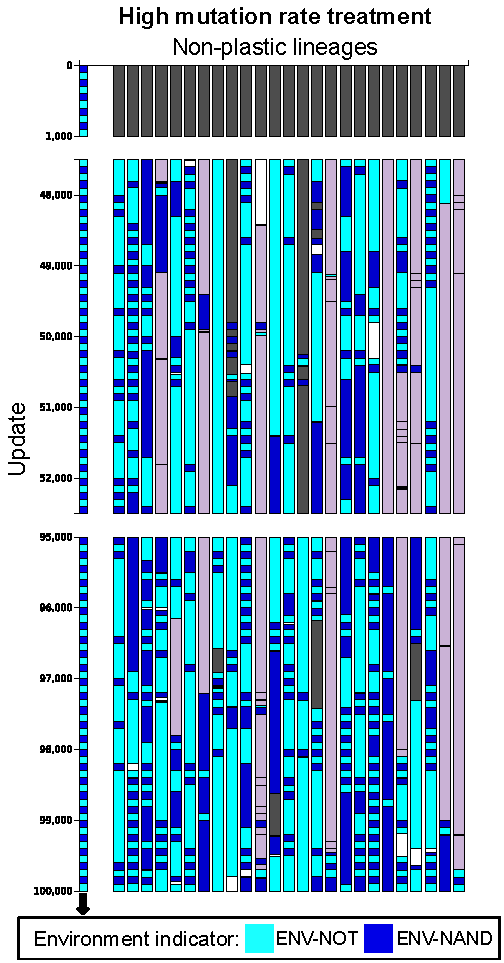
\includegraphics[height=0.5\textheight, keepaspectratio]{chapters/02-evolutionary-origins-of-plasticity/media/high-mutation-rate-non-plastic-lineages.pdf}
  \caption{\small 
  \textbf{Time-sliced visualization of lineages for non-plastic, dominant genotypes from the high-mutation-rate treatment.}
  Abbreviated color reference: 
  cyan represents unconditional NOT task performance, 
  dark blue represents unconditional NAND task performance, 
  and light purple represents sub-optimal forms of plasticity.  
  Refer to Figure \ref{chapter:origins-of-plasticity:fig:task-profiles} for a full legend of phenotype colors.}
  \label{chapter:origins-of-plasticity:fig:high-mut-lineages}
\end{figure*}



% Plastic lineages from the baseline treatment
\begin{figure*}[!ht]
  \centering
  \begin{minipage}[b]{\linewidth}
  \centering
  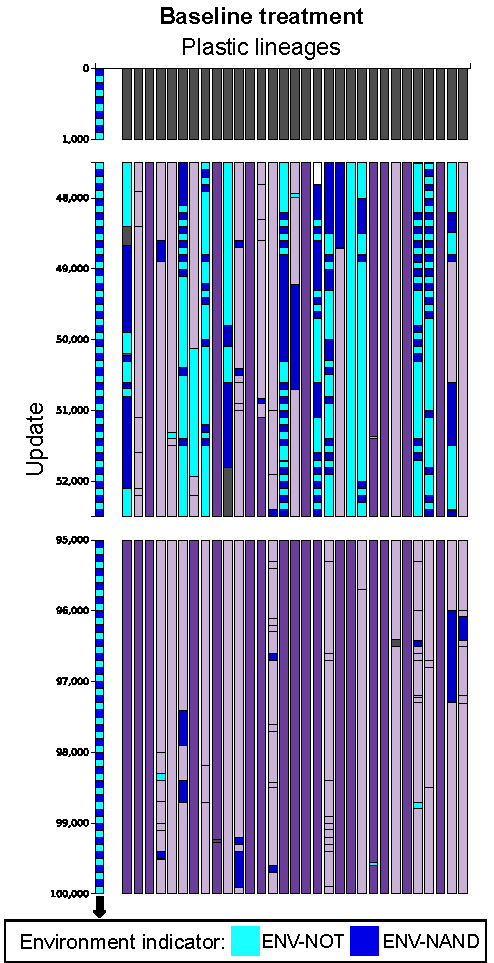
\includegraphics[height=0.5\textheight, keepaspectratio]{chapters/02-evolutionary-origins-of-plasticity/media/baseline-plastic-lineages.pdf}
  \caption{\small 
  Time-sliced lineage visualization of dominant, plastic genotypes from the baseline treatment. 
  Abbreviated color reference: 
  cyan represents unconditional NOT task performance, 
  dark blue represents unconditional NAND task performance, 
  light purple represents sub-optimal forms of plasticity, 
  and dark purple represents optimal plasticity.  
  Refer to Figure \ref{chapter:origins-of-plasticity:fig:task-profiles} for a full legend of phenotype colors.}
  \label{chapter:origins-of-plasticity:fig:baseline-lineages}
  \end{minipage}
\end{figure*}

\subsubsection{Environment Fluctuation Rate}

We found a significant difference ($p = 0.00028$ using Fisher's Exact Test with Bonferroni corrections for multiple comparisons) as we varied the cycle length for environmental switching.  
Specifically, in the long-environment-cycle-length, only 16/50 runs ended with a final dominant genotype that was phenotypically plastic, while the baseline and short-environment-cycle-length produced 31 and 36 plastic outcomes, respectively.

We expect that the short-environment-cycle-length treatment is biased toward the evolution of phenotypic plasticity because of the rapid environment fluctuations relative to other experimental treatments. 
Rapid fluctuations cause lineages to be less able to rely on mutational input for adaptation. 
In the long-environment-cycle-length treatment, environmental fluctuations may not occur rapidly enough to produce a sufficient selective pressure for phenotypic plasticity, allowing alternative adaptive strategies to evolve instead.

\subsection{What are the evolutionary stepping stones for phenotypic plasticity?}

In an attempt to identify patterns frequently encountered during the evolution of phenotypically plastic organisms, we extracted and analyzed the full lineages from our experiments. 
We tested each ancestor genotype in both ENV-NAND and ENV-NOT and classified their phenotype across both environments. 
In addition to a quantitative analysis, we also visualized the lineages of the dominant, plastic genotypes; see Figure \ref{chapter:origins-of-plasticity:fig:baseline-lineages} for the visualization of the baseline treatment. 
Using our visualizations and ancestor phenotype classifications, we addressed the following two questions: 
(1) Do the lineages of phenotypically plastic organisms first evolve to perform tasks unconditionally before evolving to perform them conditionally as a function of their current environment? 
And (2), do imperfect forms of phenotypic plasticity tend to precede optimal forms?

\subsubsection{Unconditional task performance precedes plasticity}

To explore whether or not unconditional task performance was an evolutionary stepping stone for conditional task performance (\textit{i.e.}, phenotypic plasticity), we determined whether a task was performed unconditionally prior to being performed conditionally by the ancestors of plastic genotypes. 
We analyzed both tasks (NAND and NOT) separately. These results are reported in Table \ref{chapter:origins-of-plasticity:table:evolutionary-outcomes}. 
% Answer to: unconditional before conditional?
Across all experimental treatments, non-plastic ancestors generally preceded plastic ancestors. 
In other words, unconditional task performance of the NAND and NOT tasks generally preceded the conditional performance of either task. 
Examples of this can be seen in time-sliced plastic lineages from the baseline treatment (Figure \ref{chapter:origins-of-plasticity:fig:baseline-lineages}) where many lineages maintain states of unconditional task expression prior to entering states of conditional task expression. 
These results suggest that, in fluctuating environments similar to those in our experiment, the evolutionary path to phenotypic plasticity usually traverses states of unconditional trait expression prior to entering states of conditional trait expression. 
This result should be unsurprising. 
In order to evolve a regulated function, the capacity for both the regulation and the function must exist. 
In our experiment, the function can be selected for without regulation; however, regulation of the function is unlikely to be selected for without the prior capacity for the function. 

\subsubsection{Sub-optimal plasticity precedes optimal plasticity}

To investigate sub-optimal phenotypic plasticity as an evolutionary stepping stone for optimal phenotypic plasticity in our experiment, we analyzed lineages of optimally plastic genotypes. 
Again, we consider only complete phenotypes that exclusively perform the rewarded task in each environment to be optimal. 
For each optimally plastic genotype's lineage, we determined whether or not the evolution of optimal plasticity was preceded by the evolution of sub-optimal phenotypic plasticity. 
The results of this analysis are reported in Table \ref{chapter:origins-of-plasticity:table:evolutionary-outcomes}.

% Answer to: sub-optimal before optimal?
Across all experimental treatments, the evolution of sub-optimal plasticity did, indeed, generally precede the evolution of optimal phenotypic plasticity.
Examples of sub-optimal plasticity preceding more optimal forms of plasticity can be seen in some of the time-sliced lineages from the baseline treatment visualized in Figure \ref{chapter:origins-of-plasticity:fig:baseline-lineages}. 
These results suggest that, in fluctuating environments similar to those in our experiment, sub-optimal forms of phenotypic plasticity tend to arise before the evolution of optimal forms of phenotypic plasticity. 

Unconditional trait expression tends to evolve first; then, sub-optimal forms of plasticity appear before optimal forms finally evolve.
While challenging to verify, we expect our results to be applicable to biological systems. 
The evolution of complex functions (\textit{e.g.}, optimal phenotypic plasticity) build on simpler, previously evolved functions (\textit{e.g.}, unregulated or sub-optimally regulated functions) \citep{lenski_evolutionary_2003}. 
These results, however, are particularly useful for applied evolutionary computation. 
If an evolved problem solution must respond dynamically to environmental variables, it is likely that the solution will need to be able to traverse through states of rigidity and sub-optimal plasticity prior to reaching a state of optimal plasticity. 
Thus, first evolving rigid solutions in fixed environments and then gradually starting to fluctuate more aspects of the environment over time could provide a scaffolding for the evolution of optimally plastic solutions.  

\subsection{Does plasticity still evolve when evolutionary stepping stones are disallowed?}

% Describe experiment
% - To investigate the importance of each of our observed stepping stones (unconditional trait expression and sub-optimal plasticity), we conducted a followup set of experiments.
We conducted a series of followup experiments to investigate the importance of unconditional trait expression and sub-optimal plasticity as evolutionary stepping stones.
We evolved 200 replicate populations under baseline treatment conditions (described in Section \ref{chapter:origins-of-plasticity:sec:methods:experimental-design}) and 200 replicate populations in each of three experimental conditions where we disallowed particular phenotypic profiles from evolving: (1) we disallowed phenotypes that expressed NAND and/or NOT unconditionally (\textit{i.e.}, task profiles 2, 3, and 4 from Figure \ref{chapter:origins-of-plasticity:fig:task-profiles}); (2) we disallowed sub-optimally plastic phenotypes (\textit{i.e.}, task profiles 5 through 8 and 10 through 16 from Figure \ref{chapter:origins-of-plasticity:fig:task-profiles}); and, (3) we disallowed phenotypes that exhibited unconditional trait expression \textit{or} phenotypes that were sub-optimally plastic (\textit{i.e.}, all task profiles except 1 and 9 from Figure \ref{chapter:origins-of-plasticity:fig:task-profiles}).
Note that in each of these experimental treatments, we always allowed phenotypes that expressed no tasks or were optimally plastic across both environments.
In treatments where particular phenotypes were disallowed, we tested all offspring in both ENV-NAND and ENV-NOT; if the phenotype of an organism's offspring was among the disallowed phenotypes, we prevented its birth.
As in our previous experiments, we counted the number of replicates of each treatment where the dominant genotype at the end of the experiment exhibited a plastic phenotype.
% @AML: should give each experimental treatment a name (e.g., no-unconditional-expression, no-sub-optimal-plasticity, and no-intermediate-phenotypes)

\begin{figure*}[!ht]
  \centering
  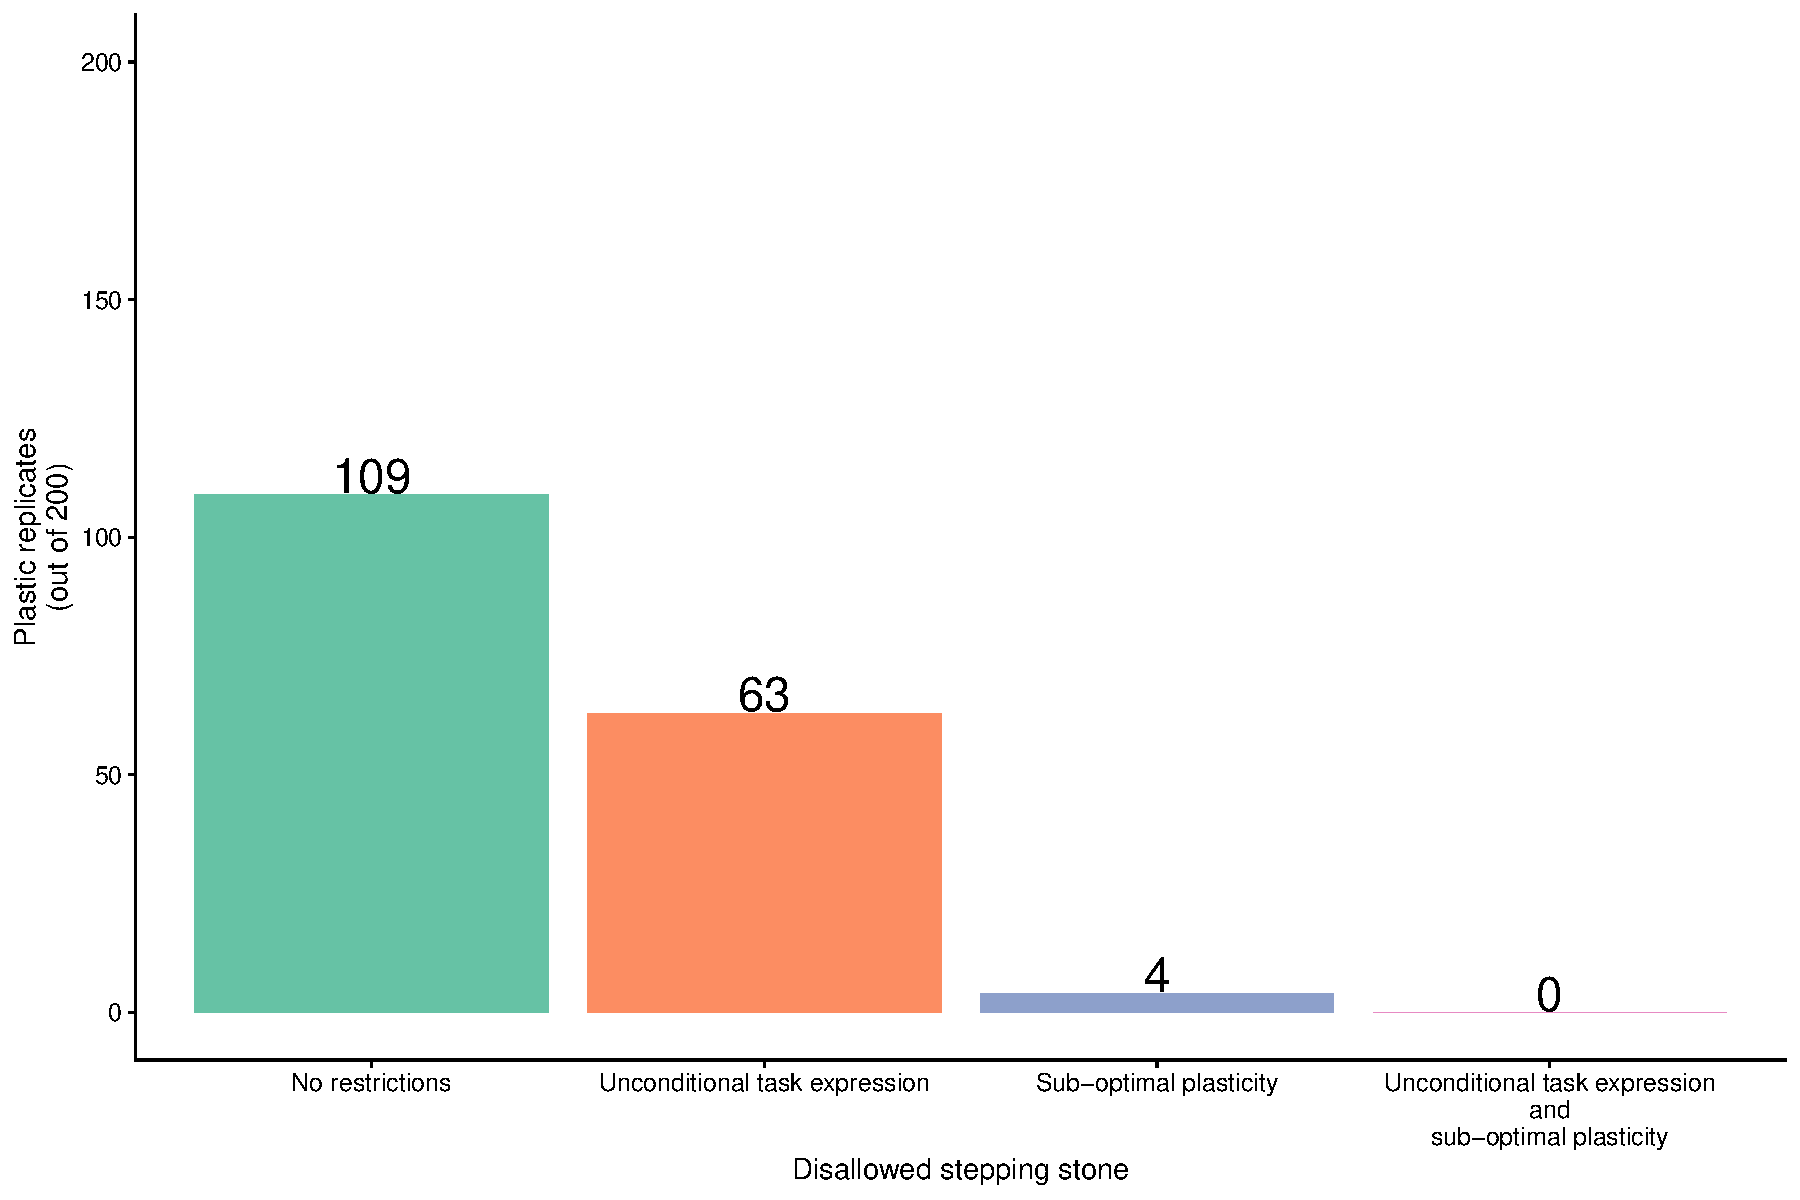
\includegraphics[height=0.3\textheight, keepaspectratio]
  {chapters/02-evolutionary-origins-of-plasticity/media/blocked-stepping-stones-baseline.pdf}
  \caption{\small A summary of evolutionary outcomes. 
  For each condition, the bar plot indicates the number of replicates (out of 200 per condition) where the final dominant genotype was plastic.
  }
  \label{chapter:origins-of-plasticity:fig:blocked-stepping-stones}
\end{figure*}

% Describe results
Figure \ref{chapter:origins-of-plasticity:fig:blocked-stepping-stones} gives the number of plastic replicates that evolved in each experimental condition.
We compared each of the three treatments that disallowed stepping stone phenotypes to our unmodified baseline treatment (Fisher's exact test with a significance level of 0.05 and a Bonferonni correction for multiple comparisons).
Each of the three treatments where we disallowed offspring with particular phenotypes had significantly fewer replicates with a plastic dominant genotype at the end of the experiment (unconditional trait expression disallowed: $p<10^{-4}$; sub-optimal plasticity disallowed: $p<10^{-4}$; both unconditional trait expression and sub-optimal plasticity disallowed: $p<10^{-4}$).

% -- Discuss --
% No intermediate phenotypes => no plasticity evolves
No phenotypically plastic genotypes evolved when we disallowed all intermediate phenotypes; when all intermediate phenotypes were disallowed, only two phenotypes were possible: (1) performing neither the NOT nor NAND tasks across environments and (2) optimally regulating between the NOT and NAND tasks across environments.
For plasticity to evolve without allowing evolution to traverse intermediate stepping stones, optimal plasticity would need arise in a single mutational step from a genotype that performed neither the NAND nor NOT tasks.
This result demonstrates that, together, these intermediate phenotypes represent crucial building blocks for the evolution of phenotypic plasticity. 

% No unconditional task expression => less plasticity
% No sub-optimal plasticity => even less plasticity
When we prevented genotypes that perform tasks unconditionally across environments, plasticity evolved less frequently than in treatments where we placed no restrictions on phenotypes; this supports our previous observation that unconditional task expression is a stepping stone toward plastic task expression. However, many replicates (63 out of 200) where unconditional task expression was disallowed still yielded plastic organisms. Thus, while unconditional trait expression is likely a valuable building block in the evolution of phenotypic plasticity, it is not necessary. Our results indicate that sub-optimal plasticity is a more important building block for optimal plasticity than unconditional trait expression. Only 4 out of 200 replicates where we disallowed sub-optimally plastic phenotypes yielded optimal plasticity. This is not unsurprising, as a lineage would need to move from a state of unconditional task expression to perfect task regulation in a single mutational step.

\subsection{Are stochastic strategies evolving as an alternative to phenotypic plasticity?}

Stochastic phenotype switching, a form of bet hedging \citep{seger_what_1987}, is a common strategy leveraged by bacteria in fluctuating environments \citep{rainey_evolutionary_2011}. 
Some forms of stochastic phenotype switching rely on mutational input to induce phenotypic changes. 
This strategy is thought to be a viable alternative to phenotypic plasticity in the absence of reliable environmental signals or when the processing of sensory information is costly \citep{rainey_evolutionary_2011}.
Strategic stochastic phenotype switching often relies on contingency loci, which are hypermutable regions of the genome that can induce phenotype switching via mutational input \citep{moxon_bacterial_2006}. 

We hypothesized that stochastic phenotype switching was an alternative evolutionary strategy to phenotypic plasticity because of its commonality in bacteria. 
We most expected to see stochastic phenotype switching in our experimental treatments where the fewest number of replicates produced phenotypically plastic final dominant genotypes. 

\subsubsection{Lineage Visualization}

It can be difficult to intuitively understand evolutionary strategies leveraged by a lineage without a visual aid.
To explore evolutionary strategies alternative to phenotypic plasticity in fluctuating environments, we visualized the lineages of dominant, non-plastic genotypes from our experimental treatments. 

\begin{figure*}[ht!]
  \centering
  \begin{minipage}[b]{\linewidth}
  \centering
  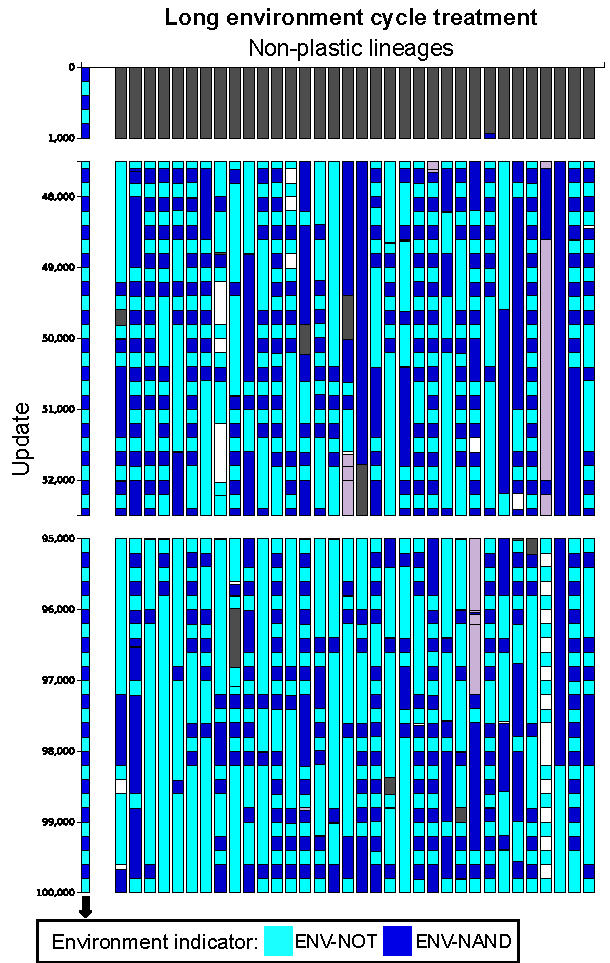
\includegraphics[height=0.4\textheight, keepaspectratio]
  {chapters/02-evolutionary-origins-of-plasticity/media/long-cycle-non-plastic-lineages.pdf}
  \caption{\small 
  Time-sliced lineage visualization of non-plastic, dominant genotypes from the long environment cycle treatment. 
  Abbreviated color reference: 
  cyan represents unconditional NOT task performance, 
  dark blue represents unconditional NAND task performance, 
  light purple represents sub-optimal forms of plasticity,
  and dark purple represents optimal plasticity. 
  Refer to Figure \ref{chapter:origins-of-plasticity:fig:task-profiles} for a full legend of phenotype colors.
  }
  \label{chapter:origins-of-plasticity:fig:long-cycle-lineages}
  \end{minipage}
\end{figure*}


If a lineage relied on stochastic phenotype switching, we would expect it to switch between phenotypic states of unconditional NAND task performance and unconditional NOT task performance in approximate synchronization with the changing environment. 
Specifically, we should see ancestors along a lineage perform NAND unconditionally during periods of ENV-NAND and see ancestors performing NOT unconditionally during periods of ENV-NOT. 
We show a time-sliced lineage visualization of dominant, non-plastic genotypes at the end of our experiment for the long-environment-cycle-length treatment (Figure \ref{chapter:origins-of-plasticity:fig:long-cycle-lineages}).  

From Figure \ref{chapter:origins-of-plasticity:fig:long-cycle-lineages}, we see what appear to be cases of stochastic phenotype switching.
That is, we observe lineages switching between phenotypic states of unconditional NAND task performance and unconditional NOT task performance in approximate synchronization with the environment. 
Many of the lineages in the long-environment-cycle treatment seem to be undergoing stochastic phenotype switching. 
A few examples of what appear to be stochastic phenotype switching can even be seen in Figure \ref{chapter:origins-of-plasticity:fig:baseline-lineages} (the plastic lineages from our baseline treatment) between updates 47,500 and 52,500 (the middle time-slice), prompting the following open question: in addition to being an alternative strategy to plasticity in fluctuating environments, could stochastic phenotype switching also act as a precursor or building block toward plasticity? 

Our visualizations only provide an exploratory method for understanding evolutionary strategies employed by a lineage. 
Further analysis would be required to confirm or reject our hypothesis that stochastic phenotype switching is evolving as an alternative strategy to phenotypic plasticity in our system. 
This hypothesis is particularly worthwhile to explore because our mutation rate was fixed across the genome, preventing the evolution of contingency loci.  
Furthermore, because sensing mechanisms were perfectly accurate, phenotypic plasticity was a reliable strategy. 
We hypothesize that genotypes are moving to a region of the mutational landscape that straddles the boundary between expressing unconditional NAND task performance and unconditional NOT task performance such that minimal mutational input is required to switch phenotypes. 
This type of evolutionary trajectory has been demonstrated by Crombach and Hogeweg in evolutionary simulations of simple, genome-encoded gene regulatory network models \citep{crombach_evolution_2008}.
In their simulations, Crombach and Hogeweg found that networks evolved in an oscillating environment possessed genotype to phenotype mappings that were mutationally more efficient at generating adaptive phenotypes in alternative environments. 
\section{Conclusion}

In this work, we evolved populations of phenotypically plastic organisms at varied rates of environmental fluctuation and mutation using the Avida Digital Evolution Platform. 
We analyzed the lineages of evolved genotypes for clues about the evolutionary stepping stones toward phenotypic plasticity. 
We found that the capacity for phenotypic plasticity evolved under conditions identified by previous research \citep{clune_investigating_2007,ghalambor_behavior_2010}. 
We found evidence that traits are generally expressed unconditionally prior to the evolution of conditional trait expression and that sub-optimal forms of phenotypic plasticity generally evolve before optimal forms of phenotypic plasticity. 
Both of these results are examples of evolution's use of simpler functions as building blocks for more complex functions as in~\cite{lenski_evolutionary_2003}. 

Visual inspection of the evolutionary histories leading to phenotypically plastic organisms suggests that under certain conditions stochastic phenotype switching evolves as an alternative strategy to phenotypic plasticity, just as it does in many bacteria \citep{moxon_bacterial_2006,rainey_evolutionary_2011}.  
Of course, in these bacterial cases, hypermutable sites tend to appear in the genomes (called ``contingency loci'') that facilitate such task switching.

Given these promising results, we plan to explore whether stochastic phenotype switching can be a viable evolutionary strategy in the absence of the ability to evolve hypermutable regions of the genome. 
Given the potential difficulty in maintaining the necessary genetic machinery associated with phenotypic plasticity, are there cases in which stochastic phenotype switching is more robust than phenotypic plasticity? 
And, does this contribute to the evolution of stochastic phenotype switching as an evolutionary strategy? 
Metrics are clearly needed for quantifying stochastic phenotype switching in digital systems and for evaluating the mutational landscapes of genotypes along a lineage. 